\documentclass[sigconf]{acmart}

\usepackage{booktabs} % For formal tables


% Copyright
\setcopyright{none}
%\setcopyright{acmcopyright}
%\setcopyright{acmlicensed}
%\setcopyright{rightsretained}
%\setcopyright{usgov}
%\setcopyright{usgovmixed}
%\setcopyright{cagov}
%\setcopyright{cagovmixed}


% DOI
\acmDOI{}

% ISBN
\acmISBN{}

%Conference
\acmConference[CSCI 599]{CSCI 599 - Blockchain Technologies}{May 2018 }{Los Angeles, California USA}
\acmYear{2018}
\copyrightyear{2018}


\acmArticle{4}
\acmPrice{15.00}

% These commands are optional
%\acmBooktitle{Transactions of the ACM Woodstock conference}
%\editor{Jennifer B. Sartor}
%\editor{Theo D'Hondt}
%\editor{Wolfgang De Meuter}


\begin{document}
\title{Scaling blockchain cryptocurrencies with leveled regions}
%\titlenote{Produces the permission block, and
%  copyright information}
%\subtitle{Extended Abstract}
%\subtitlenote{The full version of the author's guide is available as
%  \texttt{acmart.pdf} document}

\author{Eduard Sanou}
\affiliation{%
  \institution{University of Southern California}
  \city{Los Angeles}
  \state{California}
}
\email{sanou@usc.edu}

\author{Borys Gurtovyi}
\affiliation{%
  \institution{University of Southern California}
  \city{Los Angeles}
  \state{California}
}
\email{gurtovyi@usc.edu}

% The default list of authors is too long for headers.
\renewcommand{\shortauthors}{E. Sanou et al.}

% TODO
\begin{abstract}
Current blockchain based cryptocurrencies achieve very low transaction
throughputs compared to widespread transaction systems like VISA or Mastercard.
This makes current cryptocurrencies unfit to replace fiat currency.  Based on the
observation that most of the transactions\footnote{We wish to focus on
transactions performed to exchange value rather than speculative transactions
that happen in global currency trading} in a currency happen locally, and that
users of a currency are used to expect lower confirmation delays on smaller
distance transactions, we propose a way to scale a blockchain system.  Our idea
is based on a hierarchy of regions that allows transactions to happen locally
first, and non-locally afterwards following periodic intervals that increase
according to the distance.
\end{abstract}

%
% The code below should be generated by the tool at
% http://dl.acm.org/ccs.cfm
% Please copy and paste the code instead of the example below.
%
%\begin{CCSXML}
%<ccs2012>
% <concept>
%  <concept_id>10010520.10010553.10010562</concept_id>
%  <concept_desc>Computer systems organization~Embedded systems</concept_desc>
%  <concept_significance>500</concept_significance>
% </concept>
% <concept>
%  <concept_id>10010520.10010575.10010755</concept_id>
%  <concept_desc>Computer systems organization~Redundancy</concept_desc>
%  <concept_significance>300</concept_significance>
% </concept>
% <concept>
%  <concept_id>10010520.10010553.10010554</concept_id>
%  <concept_desc>Computer systems organization~Robotics</concept_desc>
%  <concept_significance>100</concept_significance>
% </concept>
% <concept>
%  <concept_id>10003033.10003083.10003095</concept_id>
%  <concept_desc>Networks~Network reliability</concept_desc>
%  <concept_significance>100</concept_significance>
% </concept>
%</ccs2012>
%\end{CCSXML}

%\ccsdesc[500]{Computer systems organization~Embedded systems}
%\ccsdesc[300]{Computer systems organization~Redundancy}
%\ccsdesc{Computer systems organization~Robotics}
%\ccsdesc[100]{Networks~Network reliability}


%\keywords{blockchain scaling, \LaTeX, text tagging}


\maketitle

% Eduard
\section{Introduction}

Current decentralized cryptocurrencies based on blockchains suffer from a
scalability problem that makes them unfit to replace centralized payment
systems such as VISA and PayPal.

We propose an idea to achieve a higher scalability than current
cryptocurrencies by creating a hierarchy of transaction regions at different
levels, in which the transactions have different properties depending on the
lowest level ancestor region.

Our first proposal is for each lowest level to work on a fork of a global
common blockchain, that would be merged with sibling zones (those under the
same parent) periodically up in the hierarchy, with the periodicity being
different at each level.  The periodicity would be lower on higher level zones.

Transactions within the lowest level zones would be applied and verified
immediately whereas those traversing zones would only be confirmed by receivers
once the forks of the corresponding zones are merged.

Our second proposal improves the efficiency of the first proposal by only
requiring transactions that cross regions to be processed at higher levels in
the hierarchy.  Each region at each level would have a separate blockchain that
would represent the underlying regions as a single \textit{superwallet}, except
for the local regions which would have a blockchain with regular wallets.

We suggest using 4 levels: Global, Country, State, City.

These designs would allow the transaction throughput within a single city to
achieve a similar throughput as current blockchains do globally.

In other words, we are optimizing transaction delays by distance, which is a
common expectation of fiat transactions, while allowing the global transaction
throughput to increase significantly.

% Borys
\section{Background}

All existing blockchain protocols have a serious limitation: scalability. It is
impossible to scale popular consensus systems such as Bitcoin because every
single node on the network processes every transaction and maintains a copy of
the entire state. The benefits of decentralization imply that every node is
independent and has equal processing requirements.

With regular database system - the solution would be very easy. We could just
add more servers - the number of servers is in direct ratio with the how system
can scale. Adding more computing power may also help but in the decentralized
world this means increasing the power of every node.  We cannot force every
participant to do so.

In fact, the blockchain actually gets weaker as more nodes are added to its
network because of the inter-node latency that logarithmically increases with
every additional node. Moreover, requirements for the node increase, and at
some point risk of centralization appears (only some part of nodes are able to
process the transaction). We end up with the trade off between throughput and
decentralization, leading to low throughput in cryptocurrencies.

\begin{table}
\centering
\begin{tabular}{l l | l l}
\textbf{System} & \textbf{tx/sec} & \textbf{System} & \textbf{tx/sec} \\
\midrule
Bitcoin & 3-4 &        Paypal &  193 \\
Ethereum & 20 &        Visa & 2,000 \\
Bitcoin Cash & 60 &          &       \\
\end{tabular}
\caption{Transaction platforms and their throughput}
\end{table}

However this is not enough to meet the needs of fiat currency.  Nowadays,
Paypal processes 193 transactions per second and Visa 2000 (with a capability
of 24,000). The majority of all transactions are local transaction (people do
fiat currency transactions locally more often than to outside places). This
fact pushed us to the idea of scaling blockchain by leveled zones.

% Eduard
\section{Scaling with leveled regions}

The main idea behind our proposal is to scale a decentralized transaction
system by removing the load nodes require to maintain the global data structure
that is the blockchain.  In order to remove this load, and thus allow an
increase of transaction throughput, we divide the the work into a hierarchy,
which for practical purposes is based on geographical regions.  The following
subsections will explain the different design choices of the system based on
the Divide and Conquer approach used in algorithm design.

\subsection{Hierarchical regions (\textit{Divide})}

The decision to use geographical regions is arbitrary, and is motivated by the
ease of understanding that the users will have upon the system, which can help
with adoption.  Other hierarchical divisions are possible with similar results;
even dynamic regions that get constantly adjusted could provide efficiency
benefits: for example, regions could be created such that all the regions in
the same level have the same amount of users, or the same amount of
computational power, or the same stake.  Nevertheless, these more efficient
divisions would make it harder for users to reason about which region they
belong to: they are less intuitive.

For our design we will use political geographical regions divided into 4
levels: Global, Country, State, City.

The reasoning behind the numbers that identify the levels is the following: the
global level is the root of the hierarchy and represents the top, so it will
have the highest number; the rest of the levels are nested and have a
decreasing decreasing number relative to their depth.  We want our system to be
flexible, and possible allow a finer level under a city (for example, big
cities could be divided into neighborhoods).  Following these constraints, we
set the global level with the identifying number of 0, and decrement by one at
each sub-level.

An important note on the divisions is that unlike other
works~\cite{unchain}light we don't require proof of location.  Regions are made
in order to divide the workload of transactions, with the idea of having local
regions working on validating and accepting transactions happening on the local
area; but this must be seen only as a convention to split the work (following
the divide and conquer strategy).  Should an attacker create identities that
claim to be in a arbitrary geographical regions, the entire system security
wouldn't be undermined.  At most the efficiency of the entire system could be
altered due to a possible unbalance of work between regions at the same level.

\subsection{Local transactions (\textit{Base case})}

Following the divide and conquer analogy, the lowest level regions (cities in
our proposal) are the smaller partition of work.  Transactions within a city
(that is, transactions where the sender and receiver belong to the same city)
are considered local, and are appended to a local blockchain, that for now, is
independent of the other cities.  This blockchain would work very similar to
current Blockchain designs, with consensus achieved through Proof of Work,
Proof of Stake, or any other proposed consensus mechanism.  The key point here
is that each city-level Blockchain will perform similarly to current Blockchain
designs, and so, globally we are increasing the total throughput by several
orders of magnitude.  Moreover, since these Blockchains have a lower number of
participants than global Blockchains, the block creation rate could be
increased rendering a much lower transaction delay than current designs.

Another possible design choice here is to use a permissioned blockchain for
each city; considering that the nodes will be in the same community could help
in the organization of such system.

\subsection{Transacting across regions (\textit{Conquer})}

If we stop here, what we would have is independent Blockchains for each city,
each representing a different currency; but we are interested in allowing
transactions across cities, across states and across countries.

\subsubsection{Forks and merges}

Our initial proposal is to start the system with a global Blockchain, common to
all regions in all levels.  This global Blockchain would be forked by the
cities and periodically merged up in the hierarchy with the forks of the
neighboring regions (at different intervals depending on the level) until
reaching the global level, at which point the process would start again
periodically.

\begin{figure}
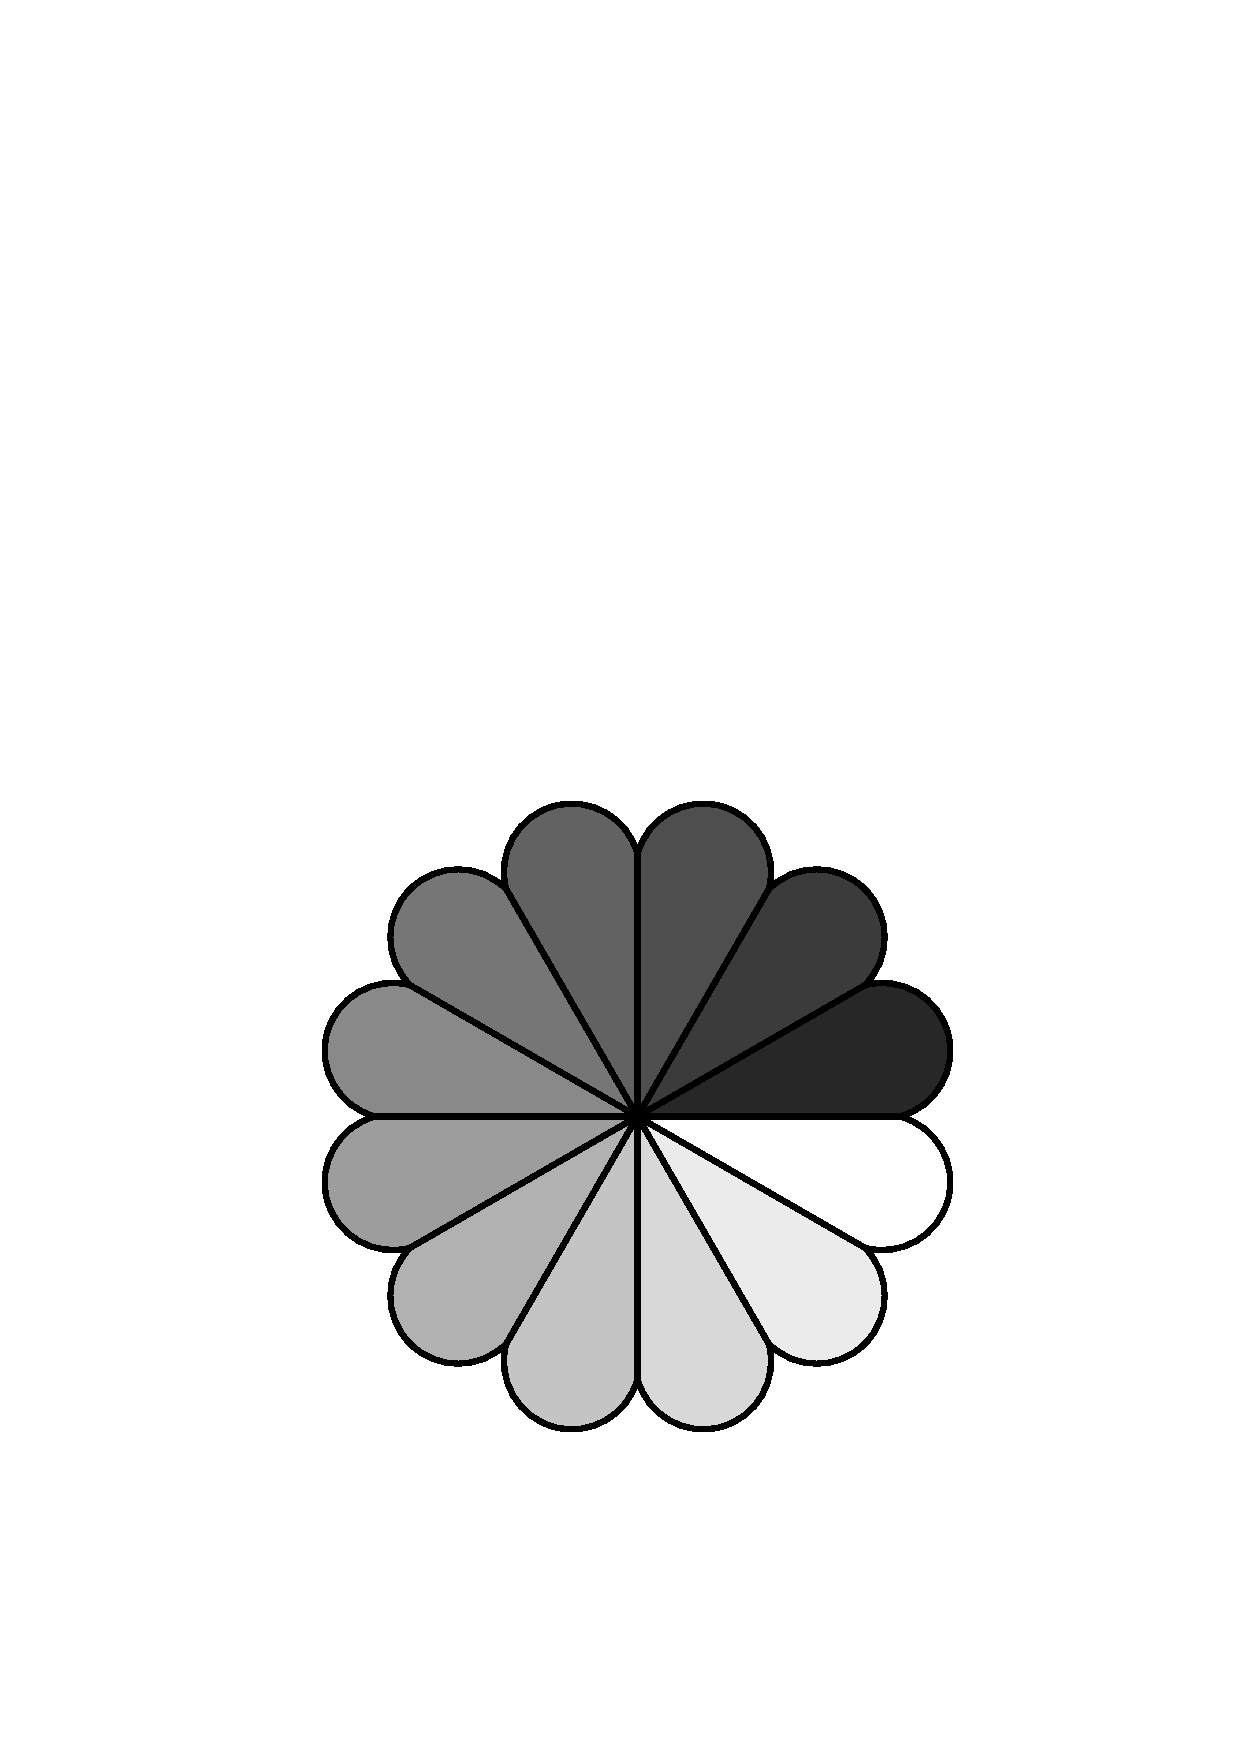
\includegraphics[height=1.8in, width=1.8in]{rosette}
\caption{Figure of forks and merges.}
\end{figure}

The following table presents a proposal for interval times for merges at each
level.  In practice, these numbers would need to be tested with a simulation of
transactions to guarantee that they are allow the merging process to happen
without overlapping with the next iteration :

\begin{table}
\centering
\begin{tabular}{l l l}
\textbf{Name} & \textbf{Level} & \textbf{periodicity}  \\
\midrule
City  &   (-3) & 10 seconds \\
State &   (-2) & 10 minutes \\
Country & (-1) & 2 hours \\
Global  & (0)  & 24 hours \\
\end{tabular}
\caption{Geographical levels and their merging periodicity}
\end{table}

Transactions made by users would only be published on the local Blockchains,
and the local community of nodes will be in charge of achieving consensus in
order to guarantee correctness for local transactions but also to have an
agreed validated list of transactions ready for the next merge with the rest of
the cities in the same state.  A rule that nodes would enforce is that they
will only accept transactions (to be added to the city local blockchain) if the
sender wallet belongs to the same city.  Assuming that each city has reached
consensus before the state merging point and that there are no
\textit{shadow}\footnote{We consider \textit{shadow} cities the case where two set of
nodes work on different blockchain forks but claim to be the same city.}
cities, the state-level merge should proceed without conflicts.

Non-local transactions would be published on the local blockchain of the
sender's wallet, but wouldn't be able to be confirmed by the receiver
immediately.  The receiver would have to wait until the sender's city fork gets
merged with their own city fork, a delay that depends on the lowest common
ancestor in the hierarchy.  The following figure shows two examples of
non-local transactions, and the required time for the receiver to be able to
confirm them.

\begin{figure}
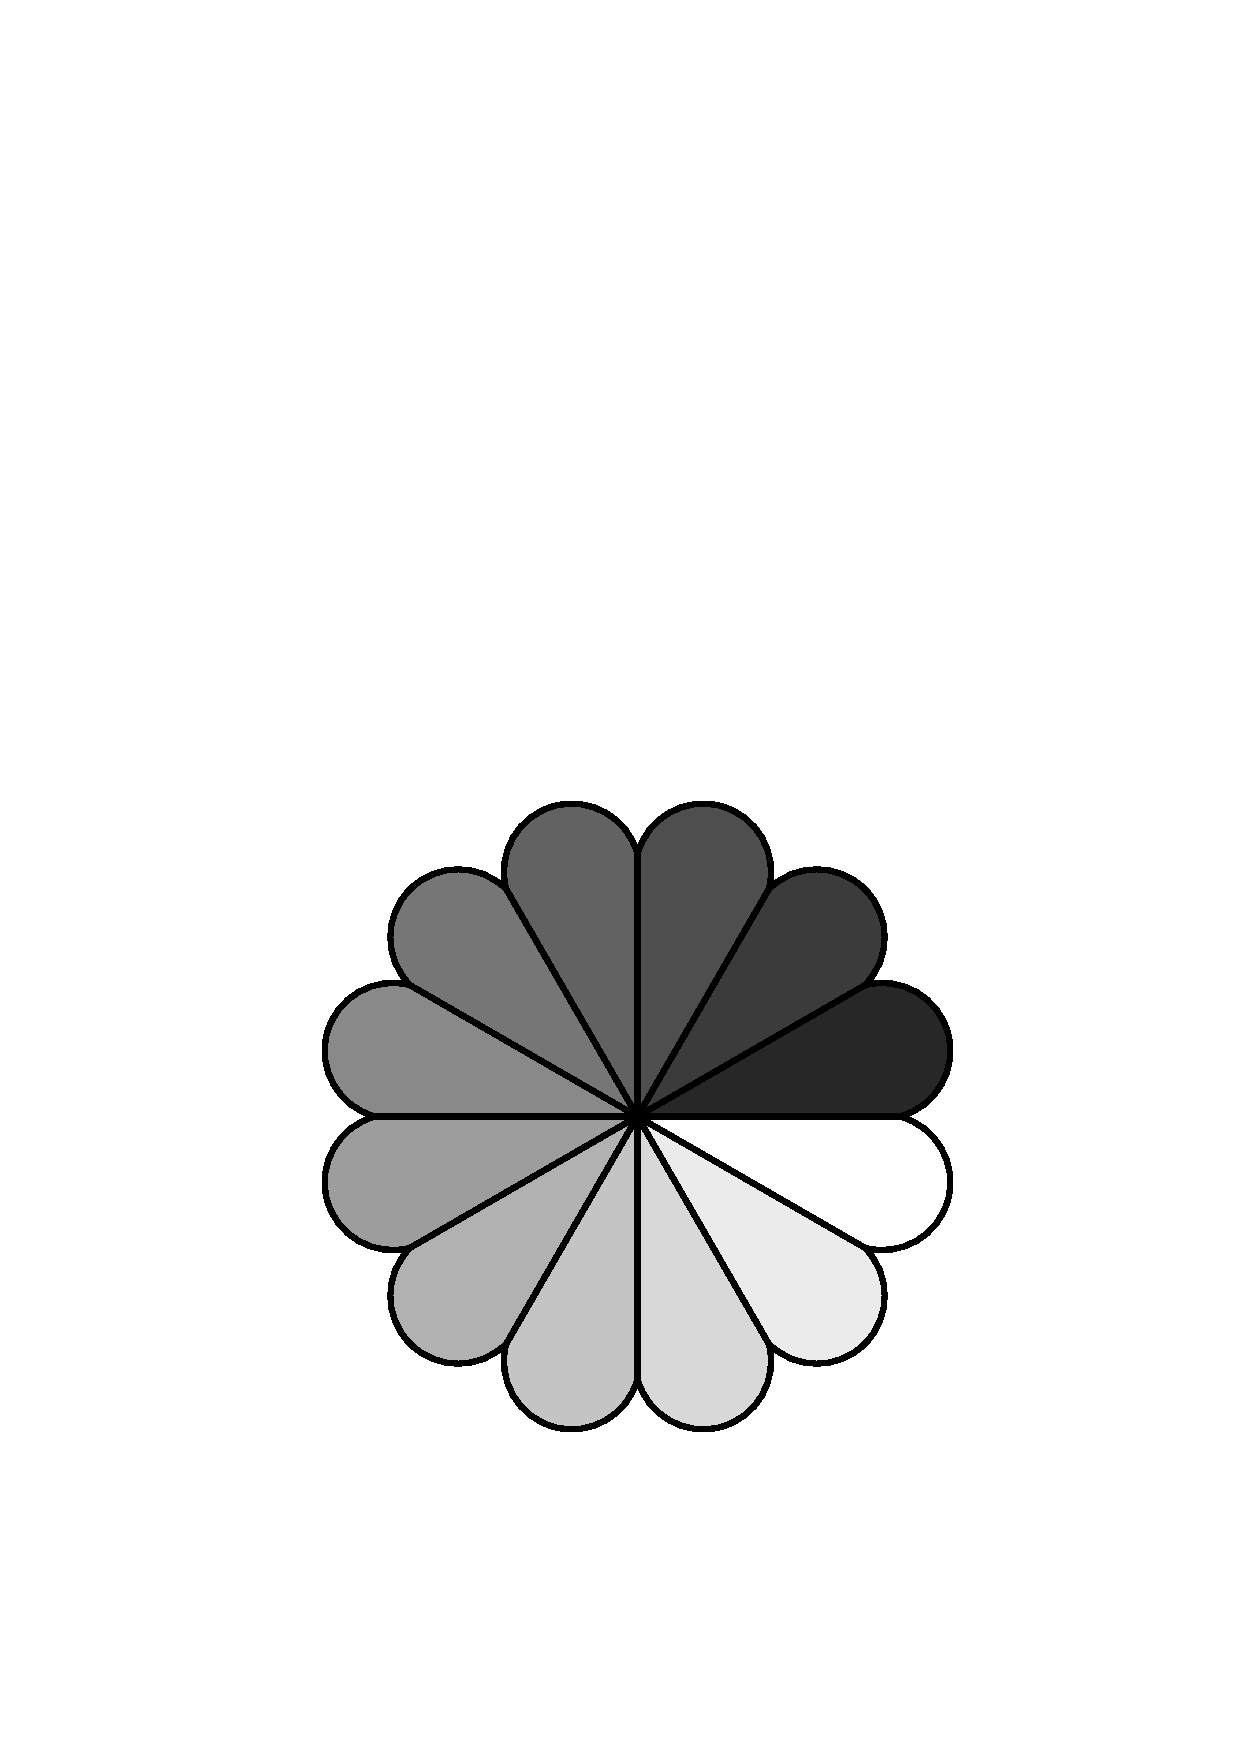
\includegraphics[height=1.8in, width=1.8in]{rosette}
\caption{Figure of non-local transactions.}
\end{figure}

For our design, blockchain city-forks would be distinguished by a tag, so that
all nodes claiming the same tag would work on the same blockchain.  Having
\textit{shadow} cities can also be seen as not reaching consensus within a city,
because it would imply disagreement under the same tag.

For wallets to belong to the same city, we introduce a special transaction that
involves wallet creation: for a wallet to be used in regular transaction, a
previous transaction which contains a city tag signed by the wallet private key
must be published.  Users traveling to a different city could create a new
wallet belonging to the new city and transfer coins to it in order to perform
local transactions in the new city; the traveler would just need to perform
this operation before traveling to avoid any friction with the system.  Like
Bitcoin and other blockchain based cryptocurrencies, each user can have as many
wallets as they desire; the only difference is that in our proposal, since a
wallet can't be used without a transaction claiming a city where it belongs,
there would probably be a small (transaction) cost associated to wallet
ownership.

\subsubsection{Using different blockchains}

The forking and merging strategy requires every node in the network to maintain
a copy of the global blockchain, which contains a big number of transactions,
thus increasing the storage requirements significantly.  Moreover, the merging
process requires a lot of bandwidth in order to synchronize the transactions
between neighboring regions, with the worst case happening at the top level
(where every country's fork merge into a global blockchain).

Considering that most of the transactions will happen locally, we could imagine
a system in which nodes aren't required to store the transaction state of the
entire system, as that information will be accessed less often.  We could
change the design so that local transactions stay in a local blockchain and are
never merged up in the hierarchy: only transactions that need to cross regions
move up and down in the tree.  This would reduce the bandwidth and storage
requirements significantly.  Furthermore, a mechanism could be engineered to
charge higher transaction costs to further distance transactions, which would
benefit users that do local transactions (and incentivize them to do so), and
compensate nodes that work on non-local transactions.

So instead of working with a global blockchain that keeps forking and merging
back following a tree; we could design the system to have a different
blockchain for each region at each level, similar to what other works have
proposed~\cite{unchain}.  The question now is how transactions go up and down
the hierarchy, and how nodes can verify the correctness of these vertical
transactions.

Our proposal for this version of the system is to maintain the local
blockchains the same way, and represent each region as a \textit{superwallet}
in the blockchain of the following upper level.  For example, transactions
between two cities would be seen as transactions between two
\textit{superwallets} in the corresponding state blockchain.  We use the notion
of \textit{superwallets} to indicate the difference between regular local
blockchain wallets: \textit{superwallets} have the characteristic that they
group many wallets underneath.  Moreover, since transactions between
\textit{superwallets} represent transactions of lower level wallets, these
transactions would need to carry extra information about the sender and
receiver of each locally originated transaction.  The following figure should
help clarifying this idea by sowing some examples of transactions in this
model:

\begin{figure}
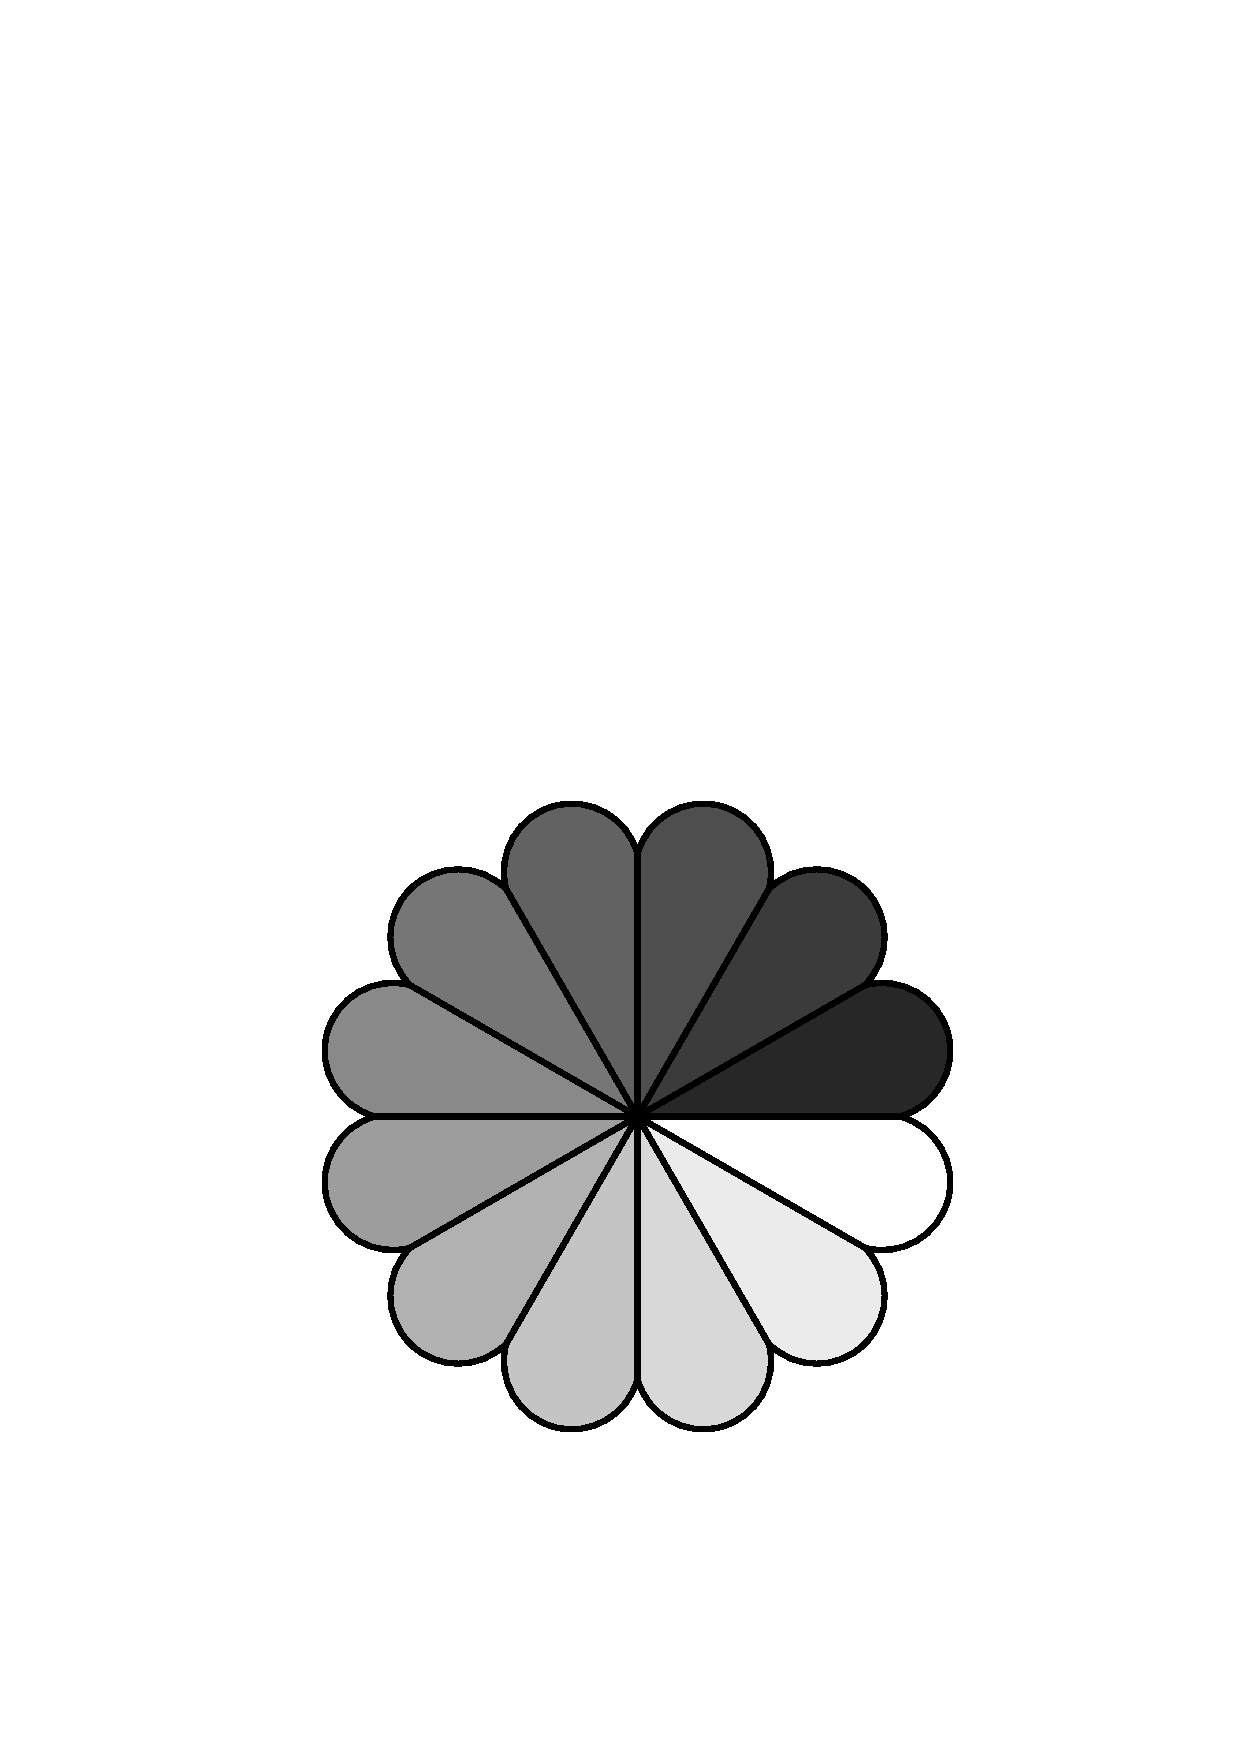
\includegraphics[height=1.8in, width=1.8in]{rosette}
\caption{Figure.}
\end{figure}

In this model, mining nodes could decide to work on the blockchains at
different levels.  Ideally, and to make things simpler, each node would work at
each level (in the corresponding nested regions it belongs to).  This would
help linking a node to a local wallet in which the node would receive the
mining rewards, which would need to be reflected in all levels to maintain
correctness (that is, because the \textit{superwallet} where the miner's wallet
belongs would increase its coin value without receiving any transaction).

% Borys
\section{Challenges/Future Work}

* The merging process requires more computational work and bandwidth on higher
levels.  Not all nodes may be capable enough to verify merges at every level,
Flexibility in the amount of contribution by node may be required.

* When a node performs a merge, it needs to verify the forks of the sibling
zones for correctness.  This could require a lot of computation resources.  A
possible optimization would be that each merge outputs a compressed form of the
result that makes verification at the next level faster.

* At the lowest level, each zone would have a small number of nodes.  This
opens the possibility of an attacker disrupting the zone by registering nodes
in it with high validation weight (either computational power or stake).  Such
disruption could be a denial of service or a denial of selected transactions.

* A way to make make sure that all zones have the same computing power could be
useful to solve this.

* A different approach would consist on restricting how easily new nodes with
high computational power can join or switch zones.

* At each level, the merging time between forks should be faster than the
periodicity of merges.

\section{Related Work}

% Eduard
\subsection{Unchain Your Blockchain}

This is a proposal~\cite{unchain} that tries to solve the current scalability
issues of public blockchain based technologies.  Very similar to our approach,
the authors design a hierarchical division based on geospatial regions.  Each
region at each level would have a different and independent blockchain such
that local transactions happen in the local blockchain associated with the
geographical area.  Farther transactions require multiple transactions to move
up and down in the hierarchy to pass through the lowest common region;
increasing the cost and delay compared to local transactions.


The authors complement this design with the idea of Proof of Location, which is
used by miners to maintain consensus of the blockchains in a fair manner and
without the power consumption associated with Proof of Work.  This design
requires an infrastructure of trusted corroborators uniformly spread over the
geographical area where the cryptocurrency is deployed.  This corroborators
consist of antennas that have the capability of issuing certificates to parties
after they have verified their proximity (by analyzing the communication
latency).  The algorithm to select which miner creates the next block in the
blockchain consist of the publication of a random corroborator antena, so that
the miner who can prove to be the closest (in distance, or latency) to the
antena wins (and gets to create the block).  Location certificates can also
improve the security from the regular users point of view by means of
geofencing their wallet, such that the coins in it can only be spent from a
particular geographical area.  The authors devise a business model behind the
corroborators by charging a fee per issued certificate, which would increase
with the distance to deter miners from getting too many of them.


The description of the system doesn't specify how correctness is verified when
crossing levels.  In single blockchain systems, each transaction is verified by
asserting that the sender has enough coins through inspection of the entire
transaction history.  It's not clear how a blockchain could verify that the
sender in a transaction from another level has enough coins, without having
access to different level blockchain.


In contrast to our proposal, the above system requires the deployment of
physical infrastructure from the corroborators, as well as trusting them in
order to function with security guarantees.  Our idea doesn't require any proof
of location, and doesn't offer any advantage to an attacker that claims to be
in a different location than their geophysical location.

% Eduard
\subsection{Payment Channels}

Payment channels are a proposal to improve the scalability of transactions by
allowing payments to happen out of the blockchain, thus increasing the total
transaction throughput and not requiring miners to process every transaction.
Rather than creating a hierarchy of transactions, this solution creates a
single off-chain protocol in which a group of parties can do an unlimited
number of transactions, which is connected to the blockchain through only two
transactions.  The first blockchain transaction is a payment that the parties
make to a chanel wallet and the second transaction is a payment from such
chanel wallet back to the participants according to the final balance of each
party in the off-chain transaction state.

Whereas initial proposals like the Lightning Network~\cite{light} or the work of
Christian Decker et.\ al.~\cite{chan1} offer solutions for just scaling
transaction throughput by allowing off-chain transactions, other works like
TumbleBit~\cite{tumble} and the work of Giulio Malavolta et.\ al.~\cite{chan2}
expand the idea by supporting anonymous payments thus increasing the privacy of
the systems.

Our proposal could be seen as an extension of payment channels, where the
channels are blockchains themselves and exist in a hierarchical tree based on
geographic regions.

% Eduard
\subsection{Plasma Project}

The authors of Ethereum have proposed the Plasma Project~\cite{plasma} which
extends the idea of off-chain transactions with smart contracts.  The proposal
involves a tree-like structure where a root blockchain has several child
blockchains that handle most of the computation and transaction load, only
using the root blockchain to store small commitments to guarantee the security
of the nested transactions.

Their system still requires nodes to verify transactions of children
blockchains, with the caveat that nodes can choose to only work on children
blockchains of interest (those that handle transactions or smart contracts that
the node cares about).  The data structure used in the root chain to secure
transactions in children blockchains is the Merkle tree.

Our idea shares some concepts with the Plasma Project, although we focus on
monetary transactions only.  In contrast to Plasma, our hierarchical tree would
be based on geographical regions.

% Borys
\subsection{Sharding}

Ethereum presented idea of sharing in their own whitepaper. The point is the
blockchain can have at most 2 to of these 3 properties: Decentralization,
Scalability, Security. Currently, transactions on the EVM are not
parallelizable, and every transaction is executed in sequence globally.

Sharing is splitting all nodes to a bunch of portions called shards. Every
shard contains its own independent state and transactions history. Every shard
contains special type of nodes called collators for storing information about
particular shard. This information has what shard is applies to, state of the
shard before/after all transaction are applied, digital signature of > 2/3 all
collators on shard which make this collation legit.

Second important type of node is supernode which is in this case responsible
for taking all collations across the shard and put them into single block. This
block will be added to blockchain.

The new block is valid if and only if all transactions in all collations are
valid, the state of the collations is same as the current state of the
collations before the transactions, the state of collations after transactions
is same as specified and 2/3 collators signed collations.  The main question
now is how to send transactions across the shards. For example A ( shard 1)
sends a 1 ETH to B (shard 2).

A transaction is sent to Shard 1 $\rightarrow$ A's balance is reduced by 1 ETH.

A receipt is created. It is not being stored in a state yet, but in the Merkle
root.

Merkle receipt with the transaction is sent to Shard 2. Balance of B is
increased by 1 ETH.

The biggest problem is a Single-Shard takeover attack. It is enough now for
attacker to take over 1 shard to start submitting invalid collations. The
Ethereum Sharding FAQ suggests random sampling of collators on each shard.

% Borys
\section{Conclusions}


\bibliographystyle{ACM-Reference-Format}
\bibliography{bibliography}

\end{document}
